% LaTeX template for Lab Reports
% Copyright (C) 2014 Julian Coy

%% CHANGE REPORT TITLE HERE
\newcommand{\reporttitle}{
 Simple Processor
}

%% HEADER/PREAMBLE INFORMATION

% "The font should be 11pt Times New Roman"
\documentclass[11pt]{report}
\usepackage[T1]{fontenc}
\usepackage[utf8]{inputenc}

\usepackage{mathptmx}               

% "The body of the paper should use 1" margins on all sides."
\usepackage[margin=1in]{geometry}

% "Pages must be numbered, starting with 1 on the first page in the body of the report.
% The cover page should not be numbered. 
% Page numbers should be in the bottom-right corner of the page."
\usepackage{fancyhdr}
\pagestyle{fancy}
\fancyhead{}
\fancyfoot{}
\renewcommand{\headrulewidth}{0pt}
\fancyfoot[R]{\thepage}

% Set up customized spacing
\usepackage{setspace}

% Allows for Trademark Symbols
\usepackage{textcomp}

% Remove spacing between items in lists
\usepackage{enumitem}

% Remove extra spacing between titles of sections and subsections
\usepackage{titlesec}
\titlespacing\section{0pt}{10pt}{10pt}
\titlespacing\subsection{0pt}{10pt}{10pt}
\titlespacing\subsubsection{0pt}{0pt plus 4pt minus 2pt}{0pt plus 2pt minus 2pt}

% Setup the specialized chapter section for the Abstract
\titlespacing\chapter{0pt}{0pt plus 4pt minus 2pt}{0pt plus 2pt minus 2pt}
\titleformat{\chapter}[block]{\centering\Huge}{}{}{}{}

% Set up BibTeX integration using IEEE citation format
\usepackage{cite}
\bibliographystyle{ieeetr}
\usepackage{url}

% Set bibliography to have a section header rather than chapter header
\makeatletter
\renewenvironment{thebibliography}[1]
     {\section*{\scshape Works Cited}% <-- this line was changed from \chapter* to \section*
      \@mkboth{\MakeUppercase\bibname}{\MakeUppercase\bibname}%
      \list{\@biblabel{\@arabic\c@enumiv}}%
           {\settowidth\labelwidth{\@biblabel{#1}}%
            \leftmargin\labelwidth
            \advance\leftmargin\labelsep
            \@openbib@code
            \usecounter{enumiv}%
            \let\p@enumiv\@empty
            \renewcommand\theenumiv{\@arabic\c@enumiv}}%
      \sloppy
      \clubpenalty4000
      \@clubpenalty \clubpenalty
      \widowpenalty4000%
      \sfcode`\.\@m}
     {\def\@noitemerr
       {\@latex@warning{Empty `thebibliography' environment}}%
      \endlist}
\makeatother

% Set up math
\usepackage{amsmath}
\usepackage{amsfonts}
\usepackage{amssymb}

% Set up graphics
\usepackage{graphicx}
\usepackage{float}

% Set up tables
\usepackage{tabularx}
\usepackage{booktabs}

% Set up code blocks
% or not...

\usepackage{listings}
\usepackage{color}

\definecolor{dkgreen}{rgb}{0,0.6,0}
\definecolor{gray}{rgb}{0.5,0.5,0.5}
\definecolor{mauve}{rgb}{0.58,0,0.82}

\lstset{frame=tb,
  language=VHDL,
  aboveskip=3mm,
  belowskip=3mm,
  showstringspaces=false,
  columns=flexible,
  basicstyle={\small\ttfamily},
  numbers=none,
  numberstyle=\tiny\color{gray},
  keywordstyle=\color{blue},
  commentstyle=\color{dkgreen},
  stringstyle=\color{mauve},
  breaklines=true,
  breakatwhitespace=true
  tabsize=3
}

%% START OF DOCUMENT

\begin{document}

% "The main body of text should use 1.5 spacing"
\begin{spacing}{1.5}

% Suppress page numbering on first page
\thispagestyle{empty}

\begin{scshape}

% Title
% "The title should be centered and written in approximately 22pt font."
\vspace*{30pt}
{
\Huge
\begin{center}
    \reporttitle
\end{center}
}
\vspace{30pt}

% Team Number
% "The Team number should be centered and written several lines below the title and should use a
% similar size font as the title."
{
\Large
\begin{center}
  Lab Report 5 for ECE327 \\
  Digital Systems Design
\end{center}
}
\vspace{30pt}
% Team Members
% "Directly below the team identifier, team members should be listed alphabetically by last name, one
% per line, in approximately 14pt font. The column of names should be approximately centered on
% the page, but the names within the column should be left justified (so they all start at the same
% horizontal position)."
{
\Large 
\begin{center}
  Submitted by \\
  Julian Coy
\end{center}
}
\vspace{120pt}

{
\Large
\begin{center}
  Undergraduate of Electrical \& Computer Engineering \\
  Clemson University
\end{center}
}
\vspace{30pt}

{
\Large
\begin{center}
  April 28, 2014
\end{center}
}

\end{scshape}

% New page and reset page numbering
\clearpage

%% START EDITS BELOW %%

\vspace{15pt}
  \setcounter{chapter}{1}
  \chapter*{Abstract}
  \label{cha:abstract}
\vspace{72pt}

Bit-pair recoding is an efficient algorithm to perform quick multiplication calculations in hardware.  The bit-pair algorithm is useful because it is guaranteed to reduce the number of shift/add operations to half of that of a normal shift/add multiplier.  The task of this lab was to implement a bit-pair recoding multiplier in VHDL code.  The entire lab was done in simulation and no actual FPGA programming was done.  The most difficult aspect of this simulation was timing between the different modules.  In order to assuage some of this issues, I implemented a clock to synchronize the operations.

\vspace{4.5in}

\textit{Note: All clocks generated for simulation were built using Morten Zilmers clock gen package \cite{Synth}.}

\thispagestyle{empty} % clear page number
\clearpage
\setcounter{page}{1}

\section*{\scshape Introduction} %(0.5 pages)
\label{cha:introduction}

The purpose of this lab is to simulate a complicated 32-bit multiplier.  The multiplier will implement the bit-pair decoding algorithm.  A diagram of the system can be seen in Figure \ref{fig:system}.  The signals, registers, and modules are labeled similarly in the code (see appendices).

\vspace{15px}
\begin{figure}[H]
    \centering
    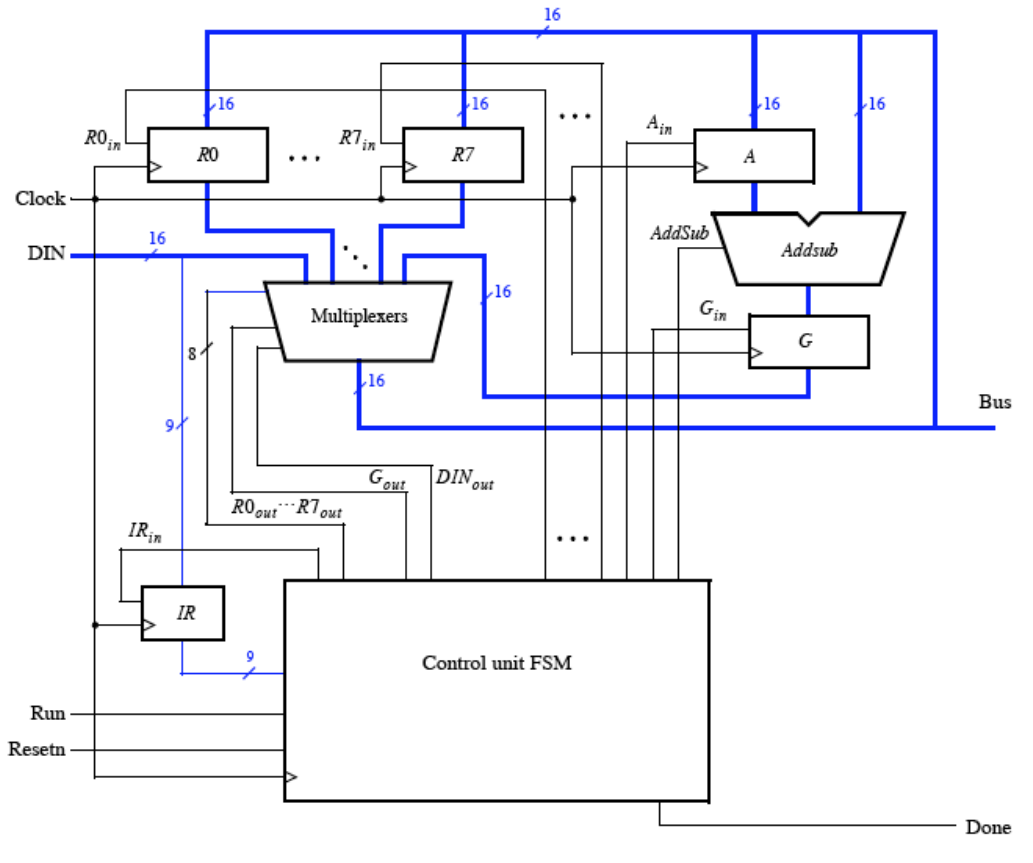
\includegraphics[width=1.0\textwidth,keepaspectratio]{system.png}
    \caption{Multiplier Circuit}
    \label{fig:system}
\end{figure}

There are five main components to this design: the control module and registers A, B, C, and D.  There is also a 32-bit adder module.  The "2-input mux" is integrated into register C and the 5-input mux is integrated into register A.  This was done to simplify the VHDL coding process.

\section{\scshape Lab 4 System Design} %(0.5 pages)
\label{sec:fsm_design}

\subsection{\scshape Register Design}
\label{sub:design_piso}

Each register is slightly different than the others.  The registers range in complexity as well.  Register A is the arguably the second most complicated register in this lab.  It stores the multiplicand and outputs the recoded version based upon the code signal (which is the lowest three bits of register B).  The output from register A is tied into the 32-bit adder.

The other line that is tied into the adder is the output from register C.  Interestingly the input from C is connected to its output.  The only way to prevent serious data integrity loss is to control when the registers load and send values.  The loadreg signal is what controls this synchronization.  Register C accepts input from the adder and will shift the results to the right by two bits.  The shifting only occurs when the shift signal is high.  The shifted values are sent into the MSBs of register B.

Register B is the closest to a "pure" register.  It only stores data and sends the lowest three bits as the code signal.  It is also capable of shifting, but instead of shifting in sign bits, register B will shift in the bits that register C just shifter out.

All of these processes and signals are controlled by the control unit.  This module is the entry point for the outside world.  It interfaces directly with register D to keep track of the calculations needed to finish multiplication.  The only signals that interface with the control unit from the outside are the start signal and the busy signal.  Once the registers are loaded (A with the multiplicand and B with the multiplier) the start signal can be set high.  This will start the multiplication process and will in turn, bring the busy signal high.  The start signal will do nothing until the busy signal is reset.  Once the busy signal is reset, register C will hold the upper 32 bits of the product and register B will hold the lower 32 bits.
\clearpage

\subsection{\scshape Testing of Register A}
\label{sub:test_piso}

Each unit was tested in groups.  This is due to the reliance of one unit upon signals from other units.  It may have been simpler to test units individually, but the method chosen proved to provide quicker results (although, debugging was more difficult).  Below are the simulation results for the different unit tests.

\vspace{15px}
\begin{figure}[H]
    \centering
    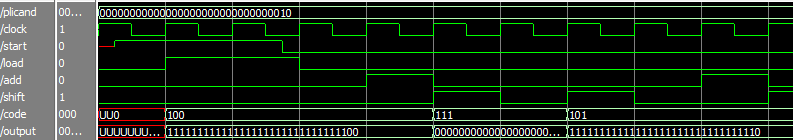
\includegraphics[width=1.0\textwidth,keepaspectratio]{rega_sim.png}
    \caption{Register A Results}
    \label{fig:rega}
\end{figure}

The test shown in Figure \ref{fig:rega} shows the manipulations that are performed on the multiplicand via register A.  Notice that as the load value goes high, the first code is produced: 100.  This code, and the following codes shown, align perfectly with the expectations for a bit-pair coding scheme.

\subsection{\scshape Testing of Registers B and D}
\label{sub:test_counter}

Registers B and D were tested at the same time to show that the counter will stop when the maximum number of shifts have occurred.  This was not necessary to do, but it aids the user in understanding why the counter is needed, as the controller has no other way of keeping track of the amount of shifts performed.

\vspace{15px}
\begin{figure}[H]
    \centering
    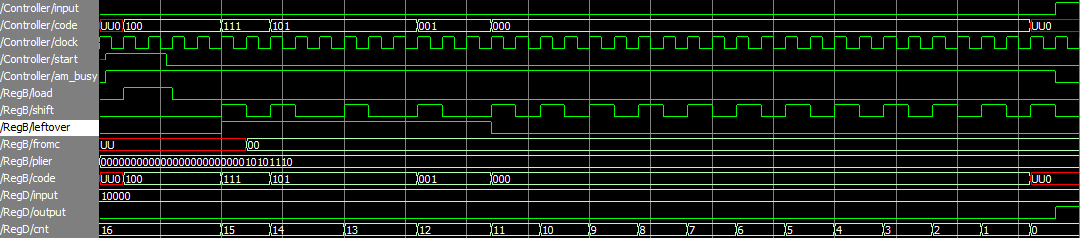
\includegraphics[width=1.0\textwidth,height=4cm,keepaspectratio]{reg_d_b.png}
    \caption{Register D and B Test}
    \label{fig:regd_b}
\end{figure}

Notice that the shifts are spaced slightly.  This occurs when an add operation is warranted.  Later on in the register C test, you will be able to see the add signal being used.  The disparity between clock cycles used per operation is the reason for the counter.  Without it there would be know way to know preemptively how many clock cycles would be needed for a given multiplication.

\subsection{\scshape Testing of Register C}
\label{sub:design_fsm}

Register C was fairly simple to implement, once the other units were designed.  In the test, you will notice that the registers values change based upon the signal changes that occur upon the signals shift, add, and load.  Register C performed the same operations as B except it did not send off the lowest three bytes for coding purposes.

\vspace{15px}
\begin{figure}[H]
    \centering
    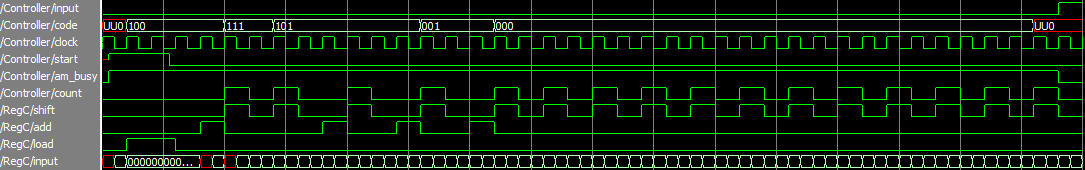
\includegraphics[width=1.0\textwidth,keepaspectratio]{reg_c.png}
    \caption{FSM State Diagram}
    \label{fig:diag_fsm}
\end{figure}

\clearpage

\section{\scshape Conclusions} % (fold)
\label{sec:conclusions}

There are definite changes that could be made to this project to increase the efficiency and decrease the overall runtime of the algorithm.  Mainly making the system asynchronous.  Do do that, more signals would need to be added to the control unit.  In particular, bus read signals would be needed to make sure register C doesn't stomp out its own value through the adder loop.

Overall, this lab shows that complex algorithms can be implemented in VHDL by creating small modules, one piece at a time.  If anything else can be taken away, it is that testing is best done on INDIVIDUAL units, not groups.  By testing entities individually, debugging is greatly simplified and overall development time and stress are reduced.

% section scshape_conclusions (end)

% Bibliography

\clearpage

\chapter*{\scshape Appendix A: Lab 4 Code}
\label{app:a}

\vspace{15px}
\begin{lstlisting}
-----------------------
--  Lab 4 Main Code  --
-----------------------

library ieee,work;
use ieee.std_logic_1164.all;
use work.all;

entity Lab4 is
  port (
    MULTIPLICAND  : in  std_logic_vector(31 downto 0);
    MULTIPLIER    : in  std_logic_vector(31 downto 0);
    START     : in  std_logic;
    CLOCK     : in  std_logic;
    BUSY      : out std_logic;
    PRODUCT     : out std_logic_vector(63 downto 0));
end entity Lab4;

architecture behav of Lab4 is
  -- Schignuls
  signal loadreg  : std_logic;
  signal shiftreg : std_logic;
  signal addreg : std_logic;
  signal count  : std_logic;
  signal code   : std_logic_vector(2 downto 0);
  signal fromc  : std_logic_vector(1 downto 0);

  signal rega_out : std_logic_vector(31 downto 0);
  signal regb_out : std_logic_vector(31 downto 0);
  signal regc_out : std_logic_vector(31 downto 0);
  signal addr_out : std_logic_vector(31 downto 0);
  signal twom_out : std_logic_vector(31 downto 0);
  signal regd_out : std_logic;

  component reg_a is
    port( load  : in    std_logic;
        plicand : in    std_logic_vector(31 downto 0);
        code  : in    std_logic_vector( 2 downto 0);
        output  : buffer  std_logic_vector(31 downto 0));
  end component reg_a;

  component reg_b is
    port( load  : in    std_logic;
        shift : in    std_logic;
        fromc : in    std_logic_vector( 1 downto 0);
        plier : in    std_logic_vector(31 downto 0);
        code  : out   std_logic_vector( 2 downto 0);
        output  : buffer  std_logic_vector(31 downto 0));
  end component reg_b;    

  component reg_c is
    port( clock : in    std_logic;
        load  : in    std_logic;
        shift : in    std_logic;
        add   : in    std_logic;
        input : in    std_logic_vector(31 downto 0);
        output  : buffer  std_logic_vector(31 downto 0);
        fromc : out   std_logic_vector( 1 downto 0));
  end component reg_c;

  component reg_d is
    port( load  : in  std_logic;
        count : in  std_logic;
        input : in  std_logic_vector(4 downto 0);
        output  : out std_logic);
  end component reg_d;

  component two_mux is
    port (  clock : in  std_logic;
        load  : in  std_logic;
        input : in  std_logic_vector(31 downto 0);
        output  : out std_logic_vector(31 downto 0));
  end component two_mux;

  component add_32 is
    port( right : in  std_logic_vector(31 downto 0);
        left  : in  std_logic_vector(31 downto 0);
        add   : in  std_logic;
        output  : out std_logic_vector(31 downto 0));
  end component add_32;

  component control is
    port( input : in  std_logic;
        code  : in  std_logic_vector(2 downto 0);
        clock : in  std_logic;
        start : in  std_logic;
        load  : out std_logic;
        shift : out std_logic;
        count : out std_logic;
        add   : out std_logic;
        busy  : out std_logic);
  end component control;

begin
  PRODUCT(63 downto 32) <= regc_out;
  PRODUCT(31 downto  0) <= regb_out;

  RegA : reg_a PORT MAP (
    load  => loadreg,
    plicand => MULTIPLICAND,
    code  => code,
    output  => rega_out
  );

  RegB : reg_b PORT MAP (
    load  => loadreg,
    shift => shiftreg,
    fromc => fromc,
    plier => MULTIPLIER,
    code  => code,
    output  => regb_out
  );

  RegC : reg_c PORT MAP (
    clock => CLOCK,
    load  => loadreg,
    shift => shiftreg,
    add   => addreg,
    input => twom_out,
    output  => regc_out,
    fromc => fromc
  );

  RegD : reg_d PORT MAP (
    load  => loadreg,
    count => count,
    input => "10000",
    output  => regd_out
  );

  TwoMux : two_mux PORT MAP (
    clock => CLOCK,
    load  => loadreg,
    input => addr_out,
    output  => twom_out
  );

  Adder : add_32 PORT MAP (
    right => rega_out,
    left  => regc_out,
    add   => addreg,
    output  => addr_out
  );

  Controller : control PORT MAP(
    input => regd_out,
    code  => code,
    clock => CLOCK,
    start => START,
    load  => loadreg,
    shift => shiftreg,
    count => count,
    add   => addreg,
    busy  => BUSY
  );

end architecture behav;
\end{lstlisting}
\clearpage
\vspace{15px}
\begin{lstlisting}
------------------------------
--  Registah Eyyyyyyyy (A)  --
------------------------------
--  i phut zee mux in zee   --
--        registah!         --
------------------------------

library ieee,work;
use ieee.std_logic_1164.all;
use ieee.numeric_std.all;
use work.all;

entity reg_a is
  port( load  : in    std_logic;
      plicand : in    std_logic_vector(31 downto 0);
      code  : in    std_logic_vector( 2 downto 0);
      output  : buffer  std_logic_vector(31 downto 0));
end entity reg_a;

architecture b_reg_a of reg_a is
begin
  loader : process (load,code)
    variable comp : std_logic_vector(31 downto 0);
  begin

    comp := not plicand; -- invert
    comp := std_logic_vector(unsigned(comp) + 1); -- add one 

    case code is
      when "000"|"111" => --  0xM
        output <= X"00000000"; -- bit 32 is unneeded but I'm weird
      when "001"|"010" => -- +1xM
        output <= plicand;
      when "011" =>   -- +2xM
        output(0) <= '0';
        output(31 downto 1) <= output(30 downto 0);
      when "100" =>   -- -2xM
        output(0) <= '0';
        output(31 downto 1) <= comp(30 downto 0);
      when "101"|"110" => -- -1xM
        output(31 downto 0) <= comp;
      when others =>
        -- ya dun &*@#ed up, son
        -- dis iz impossibru
    end case;
  end process loader;
end architecture b_reg_a;
\end{lstlisting}
\clearpage
\vspace{15px}
\begin{lstlisting}
------------------------
--  Registah Bee (B)  --
------------------------

library ieee,work;
use ieee.std_logic_1164.all;
use work.all;

entity reg_b is
  port( load  : in    std_logic;
      shift : in    std_logic;
      fromc : in    std_logic_vector( 1 downto 0);
      plier : in    std_logic_vector(31 downto 0);
      code  : out   std_logic_vector( 2 downto 0);
      output  : buffer  std_logic_vector(31 downto 0));
end entity reg_b;

architecture b_reg_b of reg_b is
  signal leftover : std_logic := '0';
begin
  loader : process (load, shift)
  begin
    if (load = '1') then
      output <= plier;
      leftover <= '0';
    end if;
    if (shift = '1') then
      leftover <= output(1);
      output(29 downto 0) <= output(31 downto 2); -- shift right by 2
      output(31 downto 30) <= fromc; -- pull in bits from reg_c
    end if;
  end process loader;

  code(2 downto 1) <= output(1 downto 0);
  code(0) <= leftover;

end architecture b_reg_b;
\end{lstlisting}
\clearpage
\vspace{15px}
\begin{lstlisting}
------------------------
--  Registah See (C)  --
------------------------

library ieee,work;
use ieee.std_logic_1164.all;
use work.all;

entity reg_c is
  port( clock : in    std_logic;
      load  : in    std_logic;
      shift : in    std_logic;
      add   : in    std_logic;
      input : in    std_logic_vector(31 downto 0);
      output  : buffer  std_logic_vector(31 downto 0);
      fromc : out   std_logic_vector( 1 downto 0));
end entity reg_c;

architecture b_reg_c of reg_c is
  signal buff : std_logic_vector(31 downto 0);
begin
  load_input : process (clock,load,add)
  begin
    if (rising_edge(clock) and (load ='1' or add ='1')) then
      buff <= input;
    end if;
  end process load_input;

  output <= buff;

  shiftah : process (clock,shift)
    variable old_bit : std_logic;
  begin
    if (rising_edge(clock) and shift = '1') then
      fromc <= buff(1 downto 0);
      old_bit := buff(31);
      buff(29 downto 0) <= buff(31 downto 2); -- buff = output >> 2
      buff(31) <= old_bit; -- sign in the bits
      buff(30) <= old_bit;
    end if;
  end process shiftah;

end architecture b_reg_c;
\end{lstlisting}
\clearpage
\vspace{15px}
\begin{lstlisting}
------------------------
--  Registah Dee (D)  --
------------------------

library ieee,work;
use ieee.std_logic_1164.all;
use ieee.numeric_std.all;
use work.all;

entity reg_d is
  port( load  : in  std_logic;
      count : in  std_logic;
      input : in  std_logic_vector(4 downto 0);
      output  : out std_logic := '0');
end entity reg_d;

architecture b_reg_d of reg_d is
  signal cnt : integer range 0 to 16 := 16;
begin
  decrement : process (count)
  begin
    if (cnt = 0) then
      output <= '1';
    elsif (count = '1') then
      cnt <= cnt - 1;
      output <= '0';
    end if;
  end process decrement;

end architecture b_reg_d;
\end{lstlisting}
\clearpage
\vspace{15px}
\begin{lstlisting}
---------------------------
--  Derty Too Bit Adduh  --
---------------------------
--  Notez:               --
--   no need for carry   --
--   out bit in mah      --
--   implementashun      --
---------------------------

library ieee,work;
use ieee.std_logic_1164.all;
use ieee.numeric_std.all;
use work.all;

entity add_32 is
  port( right : in  std_logic_vector(31 downto 0);
      left  : in  std_logic_vector(31 downto 0);
      add   : in  std_logic;
      output  : out std_logic_vector(31 downto 0));
end entity add_32;

architecture b_add_32 of add_32 is
  signal buff : std_logic_vector(31 downto 0);
begin
  adder : process (add)
  begin
    if (add = '1') then
      buff <= std_logic_vector(unsigned(left)
          + unsigned(right));
    end if;
    output <= buff;
  end process adder;
end architecture b_add_32;
\end{lstlisting}
\clearpage
\vspace{15px}
\begin{lstlisting}
--------------------------
--  Two Input Multiplex --
--------------------------
--   Two Inpuht Mucksh  -- 
--------------------------

-- this file was deemed obsolete and move into register b

library ieee,work;
use ieee.std_logic_1164.all;
use work.all;

entity two_mux is
  port (  clock : in  std_logic;
      load  : in  std_logic;
      input : in  std_logic_vector(31 downto 0);
      output  : out std_logic_vector(31 downto 0));
end entity two_mux;

architecture b_two_mux of two_mux is
  signal buff : std_logic_vector(31 downto 0) := (others => '0');
begin
  process (clock,load)
  begin
    if (rising_edge(clock) and load = '0') then
      output <= input;
    else
      output <= X"00000000";
    end if;
  end process;
end architecture b_two_mux;
\end{lstlisting}
\clearpage
\vspace{15px}
\begin{lstlisting}
--------------------------------
--  TEST BENCH CODE FOR LAB 4 --
--------------------------------

library ieee,work;
use ieee.std_logic_1164.all;
use work.clk_package.all;
use work.all;

entity test4 is --test-bench
end entity test4;

architecture behav of test4 is
  component Lab4 is
    port (
      MULTIPLICAND  : in  std_logic_vector(31 downto 0);
      MULTIPLIER    : in  std_logic_vector(31 downto 0);
      START     : in  std_logic;
      CLOCK     : in  std_logic;
      BUSY      : out std_logic;
      PRODUCT     : out std_logic_vector(63 downto 0));
  end component;

  signal plicand  : std_logic_vector(31 downto 0);
  signal plier  : std_logic_vector(31 downto 0);
  signal start  : std_logic;
  signal clockt : std_logic;
  signal busyt  : std_logic;
  signal prod   : std_logic_vector(63 downto 0);

  signal run    : std_logic := '1';

begin

  labtest : Lab4
  port map (plicand, plier, start, clockt, busyt, prod);

  clk_gen(clockt, 50.000E6, 0 fs, run);

  test : process is
  begin
    plicand <= X"00000001";
    plier <= X"00000002"; wait for 5 ns;
    start <= '1'; wait for 50 ns;
    start <= '0'; wait;
  end process;

end architecture behav;
\end{lstlisting}

%% END EDITS HERE %%

\end{spacing}

\end{document}

%%%%%%%%%%%% Extra stuff for use later

% \begin{itemize}[noitemsep,nolistsep]
%     \item \emph{Choose off-the-shelf parts} rather than self-made parts whenever possible.
%     \item \emph{Reuse and expand on open-source software libraries} to avoid spending time writing code that duplicates functionality that already exists elsewhere (and is likely more robust).
%     \item \emph{Keep the hardware simple} by using the least amount of hardware necessary for operation to avoid additional potential points of failure.
%     \item \emph{Modularize systems and components}. Each component should do one thing and do it well.
% \end{itemize}
% Figure \ref{BlockDiagram} shows a block diagram of the subsystems used in our design.

% \begin{figure}[H]
%     \centering
%     \caption{Block Diagram of Subsystems}
%     \label{BlockDiagram}
% \end{figure}
%     {
%     \centering
%       \includegraphics[width=\textwidth]{CostAccounting}
%     }